\documentclass{homework}
\usepackage{enumitem}

\newcommand{\hwclass}{Math 6108}
\newcommand{\hwname}{Jacob Hauck}
\newcommand{\hwtype}{Homework}

\newcommand{\R}{\textbf{R}}
\newcommand{\dee}{\;\text{d}}
\newcommand{\eps}{\varepsilon}
\newcommand{\pl}[2]{\frac{\partial #1}{\partial #2}}
\newcommand{\dl}[2]{\frac{\text{d} #1}{\text{d} #2}}
\newcommand{\sgn}{\text{sgn}}
\newcommand{\bigoh}{\mathcal{O}}

\usepackage{float}
\usepackage{booktabs}

\renewcommand{\hwtype}{Midterm Project}
\newcommand{\hwnum}{}
\renewcommand{\questiontype}{Problem}


\begin{document}
	\maketitle
	
	Throughout this project, we consider the IVP
	\begin{alignat}{2}
		\label{eq:ivp_ode}
		y' &= f(t, y),&\qquad &a \le t \le b\\
		\label{eq:ivp_ic}
		y(a) &= g_a,&\qquad &g_a \in \R.
	\end{alignat}
	We also use the mesh with sample points $t_j = a + jh$, with $t_0 = a$, where $h > 0$ is the step size. Lastly, we assume that $f$ is $L$-Lipschitz in $y$ uniformly for $t \in [a,b]$ (so that the solution of (\ref{eq:ivp_ode}-\ref{eq:ivp_ic}) is unique).
	
	\question
	Using the Taylor expansion for $y$ about $t_j$, we get
	\begin{equation}
		\label{p1:eq:expand_right}
		y(t_{j+1}) = y(t_j) + hy'(t_j) + \frac{h^2}{2}y''(t_j) + \bigoh(h^3).
	\end{equation}
	Similarly, expanding $y$ about $t_{j+1}$ gives
	\begin{equation}
		y(t_j) = y(t_{j+1}) - hy'(t_{j+1}) + \frac{h^2}{2}y''(t_{j+1}) + \bigoh(h^3).
	\end{equation}
	Further expanding $y''$ about $t_j$, we get
	\begin{align}
		y(t_j) &= y(t_{j+1}) - hy'(t_{j+1}) + \frac{h^2}{2}\left(y''(t_j) + \bigoh(h)\right) + \bigoh(h^3) \\
		\label{p1:eq:expand_left}
		&= y(t_{j_1}) - hy'(t_{j+1}) + \frac{h^2}{2}y''(t_j) + \bigoh(h^3).
	\end{align}
	Rearranging (\ref{p1:eq:expand_left}) and (\ref{p1:eq:expand_right}) and substituting from (\ref{eq:ivp_ode}), we get
	\begin{alignat}{2}
		\label{p1:eq:est_left}
		\frac{y(t_{j+1}) - y(t_j)}{h} &= y'(t_j) + \frac{h}{2}y''(t_j) + \bigoh(h^2)&& = f(t_j, y(t_j)) + \frac{h}{2} y''(t_j) + \bigoh(h^2), \\
		\label{p1:eq:est_right}
		\frac{y(t_{j+1}) - y(t_j)}{h} &= y'(t_{j+1}) - \frac{h}{2}y''(t_j) + \bigoh(h^2)&& = f(t_{j+1}, y(t_{j+1})) - \frac{h}{2}y''(t_j) + \bigoh(h^2).
	\end{alignat}
	If we take the average of both sides of (\ref{p1:eq:est_left}) and (\ref{p1:eq:est_right}), then we finally obtain
	\begin{equation}
		\frac{y(t_{j+1}) - y(t_j)}{h} = \frac{f(t_{j+1}, y(t_{j+1})) + f(t_j, y(t_j))}{2} + \bigoh(h^2).
	\end{equation}
	Thus, if $y_j = y(t_j)$ and we compute $y_{j+1}$ using the trapezoidal scheme, that is, as the solution of
	\begin{equation}
		\label{eq:trapezoidal}
		y_{j+1} = y_j + h\cdot\frac{f(t_{j+1}, y_{j+1}) + f(t_j, y_j)}{2},
	\end{equation}
	then $y_{j+1}$ (assuming the solution of (\ref{eq:trapezoidal}) is unique) will satisfy the estimate
	\begin{equation}
		|y_{j+1} - y(t_{j+1})| = \frac{h}{2}\cdot|f(t_{j+1}, y(t_{j+1})) - f(t_{j+1}, y_{j+1})| + \bigoh(h^3).
	\end{equation}
	Using the Lipschitz property of $f$, we obtain
	\begin{equation}
		|y_{j+1} - y(t_{j+1})| \le \frac{hL}{2}\cdot|y_{j+1} - y(t_{j+1})| + \bigoh(h^3),
	\end{equation}
	so
	\begin{equation}
		|y_{j+1}-y(t_{j+1})| \cdot\left(1 - \frac{hL}{2}\right) \le \bigoh(h^3).
	\end{equation}
	As $h \to 0$, the quantity $1 - \frac{hL}{2} \to 1$; therefore,
	\begin{equation}
		|y_{j+1} - y(t_{j+1})| = \bigoh(h^3).
	\end{equation}
	That is, the \textit{local truncation error} of the trapezoidal scheme is of order 3, which means that the \textit{global truncation error} is of order 2.
	
	\question 
	Consider the Taylor expansion of $y$ about $t_{j+1}$ at the points $t_{j-1}$, $t_j$ and $t_{j+1}$:
	\begin{align}
		y(t_{j-1}) &= y(t_{j+1}) - 2hy'(t_{j+1}) + 2h^2y''(t_{j+1}) + \bigoh(h^3) \\
		y(t_j) &= y(t_{j+1}) - hy'(t_{j+1}) + \frac{h^2}{2}y''(t_{j+1}) + \bigoh(h^3) \\
		y(t_{j+1}) &= y(t_{j+1}).
	\end{align}
	If we form the linear combination $3y(t_{j+1}) - 4y(t_j) + y(t_{j-1})$, then we get
	\begin{alignat}{2}
		3y(t_{j+1}) - 4y(t_j) + y(t_{j-1}) &{}={} &&3y(t_{j+1})\\
		&& {}-{} &4y(t_{j+1}) + 4hy'(t_{j+1}) - 2y''(t_{j+1})h^2 \\
		&&{}+{}&y(t_j)-2hy'(t_j) + 2y''(t_j)h^2 + \bigoh(h^3).
	\end{alignat}
	Therefore, canceling terms and substituting from (\ref{eq:ivp_ode}), we have
	\begin{equation}
		3y(t_{j+1}) - 4y(t_j) + y(t_{j-1}) = hf(t_{j+1}, y(t_{j+1})) + \bigoh(h^3)
	\end{equation}
	Thus, if we know that $y_{j-1} = y(t_{j-1})$, and $y(t_j) = y_j$ and we compute $y_{j+1}$ using the two-step backward differentiation scheme, that is, as the solution of
	\begin{equation}
		\label{p2:eq:2_step_backward}
		\frac{3y_{j+1} -4t_j + y_{j-1}}{2h} = hf(t_{j+1},y_{j+1}),
	\end{equation}
	then the local truncation error $|y_{j+1} - y(t_{j+1})|$ will satisfy
	\begin{equation}
		|y_{j+1} - y(t_{j+1})| = h|f(t_{j+1}, y_{j+1}) - f(t_{j+1}, y(t_{j+1}))| + \bigoh(h^3).
	\end{equation}
	By the Lipschitz property of $f$,
	\begin{equation}
		|y_{j+1} - y(t_{j+1})| \le hL|y_{j+1}-y(t_{j1+})| + \bigoh(h^3),
	\end{equation}
	so
	\begin{equation}
		|y_{j+1} - y(t_{j+1})|(1-hL) \le \bigoh(h^3).
	\end{equation}
	As $h \to 0$, the quantity $(1-hL) \to 1$; therefore,
	\begin{equation}
		|y_{j+1} - y(t_{j+1})| = \bigoh(h^3).
	\end{equation}
	That is, the \textit{local trunction error} of the two-step backward differentiation scheme is of order 3, and the \textit{global truncation error} is of order 2.
	
	\question
	Consider the Taylor expansions of $y(t_{j+1})$, $y(t_j)$, $y(t_{j-1})$, and $y(t_{j-2})$ about $t_{j+1}$:
	\begin{align}
		y(t_{j+1}) &= y(t_{j+1}) \\
		y(t_j) &= y(t_{j+1}) - hy'(t_{j+1}) + \frac{h^2}{2}y''(t_{j+1}) - \frac{h^3}{6}y'''(t_{j+1}) + \bigoh(h^4) \\
		y(t_{j-1}) &= y(t_{j+1}) - 2hy'(t_{j+1}) + 2h^2y''(t_{j+1}) - \frac{4h^3}{3}y'''(t_{j+1}) + \bigoh(h^4) \\
		y(t_{j-2}) &= y(t_{j+1}) - 3hy'(t_{j+1}) + \frac{9h^2}{2}y''(t_{j+1}) - \frac{9h^3}{2}y'''(t_{j+1}) + \bigoh(h^4)
	\end{align}
	Then, for $\beta_1, \beta_2, \beta_3, \beta_4 \in \R$,
	\begin{align}
		\beta_1 y(t_{j+1}) + \beta_2 y(t_j) &+ \beta_3 y(t_{j-1}) + \beta_4 y(t_{j-2}) = \\
		&\quad(\beta_1 + \beta_2+ \beta_3 + \beta_4)y(t_{j+1}) \\ &- (\beta_2 + 2\beta_3 + 3\beta_4)y'(t_{j+1})h \\ &+ \frac{1}{2}(\beta_2 + 4\beta_3 + 9\beta_4)y''(t_{j+1})h^2 \\ &- \frac{1}{6}(\beta_2 + 8\beta_3 + 27\beta_4)y'''(t_{j+1})h^3 + \bigoh(h^4).
	\end{align}
	To cancel the lower-order terms, we must choose $\beta_2$, $\beta_3$, and $\beta_4$ such that
	\begin{equation}
		\label{p3:eq:beta_requirements}
		\begin{aligned}
			-1 &= \beta_2 + \beta_3 + \beta_4 \\
			0 &= \beta_2 + 4\beta_3 + 9\beta_4 \\
			0 &= \beta_2 + 8\beta_3 + 27\beta_4,
		\end{aligned}
	\end{equation}
	then we get
	\begin{equation}
		\label{p3:eq:three_step_bdf_est}
		\frac{y(t_{j+1}) + \beta_2y(t_j) + \beta_3y(t_{j-1}) + \beta_4y(t_{j-2})}{-(\beta_2 + 2\beta_3 + 3\beta_4)h} = y'(t_{j+1}) + \bigoh(h^4) = f(t_{j+1}, y(t_{j+1})) + \bigoh(h^3).
	\end{equation}
	To satisfy (\ref{p3:eq:beta_requirements}), we must have $4\beta_3 + 9\beta_4 = 8\beta_3 + 27\beta_4$, so $\beta_3 = -\frac{9}{2}\beta_4$. Then $\beta_2 = 18\beta_4 - 9\beta_4 = 9\beta_4$, and $-1 = 9\beta_4 - \frac{9}{2}\beta_4 + \beta_4 = \frac{11}{2}\beta_4$, so $\beta_4 = -\frac{2}{11}$. Then $\beta_3 = \frac{9}{11}$, and $\beta_2 = -\frac{18}{11}$. Lastly, $-(\beta_2 + 2\beta_3 + 3\beta_4) = \frac{6}{11}$.
	
	If we set 
	\begin{align}
		\alpha_1 &= \frac{1}{-(\beta_2 + 2\beta_3 + 3\beta_4)} = \frac{11}{6} \\
		\alpha_2 &= \frac{\beta_2}{-(\beta_2 + 2\beta_3 + 3\beta_4)} = -\frac{18}{6}\\
		\alpha_3 &= \frac{\beta_3}{-(\beta_2 + 2\beta_3 + 3\beta_4)} = \frac{9}{6}\\
		\alpha_4 &= \frac{\beta_4}{-(\beta_2 + 2\beta_3 + 3\beta_4)} = -\frac{2}{6},
	\end{align}
	then by (\ref{p3:eq:three_step_bdf_est}),
	\begin{equation}
		\frac{\alpha_1y(t_{j+1}) +\alpha_2y(t_j) +\alpha_3y(t_{j-1}) + \alpha_4y(t_{j-2})}{h} = f(t_{j+1},y(t_{j+1})) + \bigoh(h^3).
	\end{equation}
	If we had $y_{j-2} = y(t_{j-2})$, $y_{j-1} = y(t_{j-1})$, and $y_j = y(t_j)$, and we computed $y_{j+1}$ as the solution of
	\begin{equation}
		\frac{\alpha_1y_{j+1} + \alpha_2y_j +\alpha_3y_{j-1} + \alpha_4y_{j-2}}{h} = f(t_{j+1}, y_{j+1}),
	\end{equation}
	then $|y_{j+1} - y(t_{j+1})|$ would satisfy
	\begin{equation}
		|y_{j+1} - y(t_{j+1})| = \frac{h}{\alpha_1}\cdot|f(t_{j+1}, y_{j+1}) - f(t_{j+1}, y(t_{j+1}))| + \bigoh(h^4).
	\end{equation}
	Using the Lipschitz property of $f$, we obtain
	\begin{equation}
		|y_{j+1} - y(t_{j+1})|\cdot\left(1-\frac{hL}{\alpha_1}\right) \le \bigoh(h^4).
	\end{equation}
	As $h\to 0$, the quantity $1-\frac{hL}{\alpha_1} \to 1$; therefore,
	\begin{equation}
		|y_{j+1} - y(t_{j+1})| = \bigoh(h^4).
	\end{equation}
	That is, the implicit scheme
	\begin{equation}
		\label{p3:eq:3_step_bdf_scheme}
		\frac{\alpha_1y(t_{j+1}) + \alpha_2y(t_j) +\alpha_3y(t_{j-1}) + \alpha_4y(t_{j-2})}{h} = f(t_{j+1}, y_{j+1})
	\end{equation}
	with $\alpha_1 = \frac{11}{6}$, $\alpha_2 = -\frac{18}{6}$, $\alpha_3 = \frac{9}{6}$, and $\alpha_4 = -\frac{2}{6}$ has 3rd-order global accuracy and 4th order local accuracy. Since we had to choose these values of $\alpha$ to cancel higher-order terms, these must be the coefficients in the third-order backward differentiation scheme.
	\\
	\hrule
	
	We now consider Newton's method for finding the root of a function $f$:
	\begin{equation}
		x_{k+1} = x_k - \frac{f(x_k)}{f'(x_k)}.
	\end{equation}
	
	\question
	Suppose that $f$ has a root $z$ of multiplicity $m \ge 2$. Then, by definition, there exists a function $r$ such $r(z) \ne 0$, and $f(x) = (x-z)^mr(x)$. Then $f'(x) =m(x-z)^{m-1}r(x) + (x-z)^mr'(x) = (x-z)^{m-1}(mr(x) + (x-z)r'(x))$. Then we can still safely define Newton's method despite the fact that $f'(z) = 0$ by setting
	\begin{equation}
		g(x) = x - \frac{f(x)}{f'(x)} = x - \frac{(x-z)^mr(x)}{(x-z)^{m-1}(mr(x) + (x-z)r'(x))} = x- \frac{(x-z)r(x)}{mr(x) + (x-z)r'(x)}
	\end{equation}
	and observing that the denominator in the last expression is nonzero when $x =z$ because $r(z) \ne 0$. Then Newton's method becomes $x_{k+1} = g(x_k)$.
	
	To apply the theory of convergence in the project description, we need to compute
	\begin{equation*}
		g'(x) = 1 - \frac{(r(x) + (x-z)r'(x))(mr(x) + (x-z)r'(x)) - (x-z)r(x)(mr'(x) + r'(x) + (x-z)r''(x))}{(mr(x) + (x-z)r'(x))^2}
	\end{equation*}
	so that
	\begin{equation}
		g'(z) = 1 - \frac{m(r(z))^2}{(mr(z))^2} = 1 - \frac{1}{m}
	\end{equation}
	since $r(z) \ne 0$. Since $g'(z) \ne 0$ if $m \ge 2$, but $|g'(z)| < 1$, it follows by the convergence theorem in the project description that Newton's method has \textit{linear} convergence in this case.
	
	\question
	In the case that $f$ has a root $z$ of multiplicity $m \ge 2$, we saw that Newton's method defined by $x_{k+1} = g(x_k)$, where
	\begin{equation}
		g(x) = x - \frac{(x-z)r(x)}{mr(x) + (x-z)r'(x)}
	\end{equation}
	had a linear convergence rate to the root $z$ of $f$. We can fix this simply by adjusting Newton's method to
	\begin{equation}
		x_{k+1} = x_k - m\frac{f(x_k)}{f'(x_k)},
	\end{equation}
	that is, by replacing $g$ by $g_m$, where
	\begin{equation}
		g_m(x) = x - m\frac{(x-z)r(x)}{mr(x) + (x-z)r'(x)}.
	\end{equation}
	This method has at least quadratic convergence by the convergence theorem in the project description because
	\begin{equation*}
		g_m'(x) = 1 - m\frac{(r(x) + (x-z)r'(x))(mr(x) + (x-z)r'(x)) - (x-z)r(x)(mr'(x) + r'(x) + (x-z)r''(x))}{(mr(x) + (x-z)r'(x))^2}
	\end{equation*}
	so that
	\begin{equation}
		g_m'(z) = 1-  m\frac{m(r(z))^2}{(mr(z))^2} = 0.
	\end{equation}
	Then the iteration $x_{k+1} = g_m(x_k)$ converges at least quadratically to the root $z$ of $f$ by the convergence theorem in the project description.
	\\
	\hrule
	
	Now we consider the implementation of the backward Euler method for (\ref{eq:ivp_ode}, \ref{eq:ivp_ic}):
	\begin{equation}
		y_0 = y(a) = g_a, \qquad y_{j+1} = y_j + hf(t_{j+1}, y_{j+1}) \quad\text{if}\quad j \in \{0,1,\dots, J-1\}.
	\end{equation}
	
	\question
	\newcommand{\newf}{\tilde{f}}
	\newcommand{\newg}{\tilde{g}}
	Suppose that $y_j$, $t_{j+1}$ and $h$ are known at the $j$th step of the backward Euler method. Then $y_{j+1}$ can be obtained by solving the nonlinear equation
	\begin{equation}
		\label{eq:p6:equation_to_solve}
		y_{j+1} = y_j + hf(t_{j+1}, y_{j+1})
	\end{equation}
	for $y_{j+1}$. Since our methods for numerically solving nonlinear equations work only for equations of the form $\newf(x) = 0$ (for the bisection, Netwton's and secant methods) and $\newg(x) = x$ (for the fixed point method), we need to recast (\ref{eq:p6:equation_to_solve}) in these forms. In other words, we need to define $\newf$ and $\newg$ such that
	\begin{equation}
		\newf(y_{j+1}) = 0 \iff y_{j+1} = y_j + hf(t_{j+1}, y_{j+1}) \iff \newg(y_{j+1}) = y_{j+1}.
	\end{equation}
	There are many ways to do this, but perhaps the simplest is to choose
	\begin{equation}
		\newf(x) = x - y_j - hf(t_{j+1}, x),\qquad \newg(x) = y_j + hf(t_{j+1}, x).
	\end{equation}
	
	\question
	Suppose that we wanted to use the bisection method or the secant method to solve $x = y_j + hf(t_{j+1}, x)$ for $x$.
	\begin{alphaparts}
		\questionpart To use the bisection method, we would need to know
		\begin{enumerate}[label=(\arabic*)]
			\item the initial interval $[a,b]$ that contains the root, and
			\item the stopping conditions (error tolerances and maximum iterations).
		\end{enumerate}
		As mentioned in the project description, the stopping conditions can be set according to the accuracy requirements determined by the step size $h$. The initial interval, however, would be more difficult to determine.
		
		\questionpart
		To use the secant method, we would need to know
		\begin{enumerate}[label=(\arabic*)]
			\item the initial points $x_0$ and $x_1$, and
			\item the stopping conditions (error tolerances and maximum iterations).
		\end{enumerate}
		As with the bisection method, the stopping conditions here can be determined fairly easily. The two initial points, however, would be more difficult to choose. Perhaps $x_0 = y_{j-1}$ and $x_1 = y_j$ would work, but we would still need to answer the question of how to choose $x_0$ when $j=0$.
	\end{alphaparts}
	
	\question
	In this problem, we attempt to use the backward Euler method to solve the following special case of (\ref{eq:ivp_ode}, \ref{eq:ivp_ic}):
	\begin{equation}
		\label{eq:p8:ode}
		y' = e^{2t}y^2, \qquad y(0) = 0.1, \qquad 0\le t\le 1.
	\end{equation}
	\begin{alphaparts}
		\questionpart
		\newcommand{\solver}{\mathrm{solver}}
		In order to avoid duplicate code, I have implemented an abstract version of the backward Euler method that takes as input the initial condition $g_a$, the interval $[a,b]$, and the step size $h$. The function $f$ is specified implicitly by the function argument $\solver$, defined by
		\begin{equation}
			\solver(x_0, t, h) = \text{solution $x$ of } \big[x = x_0 + hf(t,x)\big].
		\end{equation}
		I define two solver functions, one that uses Newton's method, and one that uses the fixed point method. 
		
		In Listing \ref{lst:backward_euler} is the abstract backward Euler method implementation (copied from \verb*|backward_euler.m|). In Listings \ref{lst:be_newton} and \ref{lst:be_fixed} (copied from \verb*|be_newton.m| and \verb*|be_fixed.m|) are functions that construct suitable $\solver$ functions that use Newton's method and the fixed point method to solve the equation $x = x_0 + hf(t,x)$ for $x$ by converting the equation into $\newf(x) = 0$ and $\newg(x) = x$, where $\newf$ and $\newg$ are the same as in Problem 6; note that we need to take $x_0 = y_j$ and $t = t_{j+1}$ so that $\newf(x) = 0$ and $\newg(x) = x$ are equivalent to $x = x_0 + hf(t,x)$ (see line 16 of Listing \ref{lst:backward_euler}).
		
		\lstinputlisting[language=MATLAB, numbers=left, frame=single, basicstyle=\small\ttfamily, showstringspaces=false, caption={Abstract backward Euler method}, label=lst:backward_euler]{backward_euler.m}
		
		\lstinputlisting[language=MATLAB, numbers=left, frame=single, basicstyle=\small\ttfamily, showstringspaces=false, caption={$\solver$ using Newton's method}, label=lst:be_newton]{be_newton.m}
		
		\lstinputlisting[language=MATLAB, numbers=left, frame=single, basicstyle=\small\ttfamily, showstringspaces=false, caption={$\solver$ using the fixed point method}, label=lst:be_fixed]{be_fixed.m}
		
		The two types of $\solver$ constructed by \verb*|be_newton| and \verb*|be_fixed| call the \verb*|newton| and \verb*|fixed| functions, which implement Newton's method and the fixed point method and were defined in Homework 1 and 2. For reference, they can be found in Listings \ref{lst:newton} and \ref{lst:fixed} (copied from \verb*|newton.m| and \verb*|fixed.m|. I modified them slightly for this project -- they no longer output the state at each iteration step, but now provide an option to log the total number of steps, which we will need later).
		
		\lstinputlisting[language=MATLAB, numbers=left, frame=single, basicstyle=\small\ttfamily, showstringspaces=false, caption={Newton's method}, label=lst:newton]{newton.m}
		\lstinputlisting[language=MATLAB, numbers=left, frame=single, basicstyle=\small\ttfamily, showstringspaces=false, caption={The fixed point method}, label=lst:fixed]{fixed.m}
		
		\questionpart 
		In Table \ref{table:p8:b} (summarized from \verb*|p8_output.txt|) are the numerical values of $y(1)$ (that is, $y_J$) output by the backward Euler method using Newton's method and the fixed point method for the nonlinear equation, with step size $h \in \left\{\frac{1}{4}, \frac{1}{8}, \frac{1}{16}, \frac{1}{32}, \frac{1}{64}, \frac{1}{128}\right\}$.
		\begin{table}[H]
			\centering
			\begin{tabular}{@{}lll@{}}
				\toprule
				& \multicolumn{2}{c}{$y_J$} \\
				\cmidrule{2-3}
				$h$ & Fixed & Newton \\
				\midrule
				$\frac{1}{4}$ & 0.235418015201 & 0.235440531032 \\[0.4em]
				$\frac{1}{8}$ & 0.165331430895 & 0.165335563041 \\[0.4em]
				$\frac{1}{16}$ & 0.154566102258 & 0.154571002483 \\[0.4em]
				$\frac{1}{32}$ & 0.150463955586 & 0.150469141443 \\[0.4em]
				$\frac{1}{64}$ & 0.148618358067 & 0.148639382119 \\[0.4em]
				$\frac{1}{128}$ & 0.147724451062 & 0.147777319070 \\[0.4em]
				\bottomrule
			\end{tabular}
			\caption{Backward Euler $y_J$ values}
			\label{table:p8:b}
		\end{table}
		
		\questionpart
		We can solve (\ref{eq:p8:ode}) directly by separation of variables.
		\begin{equation}
			\frac{y'}{y^2} = e^{2t} \implies -y^{-1} = \frac{1}{2}e^{2t} + C,
		\end{equation}
		where $C$ is a constant. Since $y(0) = .1$, it follows that $-10 = \frac{1}{2} + C$, so $C = -\frac{21}{2}$. Therefore,
		\begin{equation}
			y(t) = \frac{2}{21- e^{2t}}
		\end{equation}
		is the solution of (\ref{eq:p8:ode}).
		
		In Table \ref{table:p8:c} (summarized from \verb*|p8_output.txt|) are the errors between $y(1)$ and the numerical approximation $y_J$ output by the backward Euler method using Newton's method and the fixed point method for the nonlinear equation, with step size $h \in \left\{\frac{1}{4}, \frac{1}{8}, \frac{1}{16}, \frac{1}{32}, \frac{1}{64}, \frac{1}{128}\right\}$.
		
		We see that the error decreases by a factor of roughly $2$ each time $h$ decreases by a factor of $2$. This is consistent with backward Euler method's linear convergence: $|y_J - y(1)| = \bigoh(h)$.
		\begin{table}[H]
			\centering
			\begin{tabular}{@{}lll@{}}
				\toprule
				& \multicolumn{2}{c}{$|y(1) - y_J|$} \\
				\cmidrule{2-3}
				$h$ & Fixed & Newton \\
				\midrule
				$\frac{1}{4}$ & 8.847743e-02 & 8.849995e-02 \\[0.4em]
				$\frac{1}{8}$ & 1.839085e-02 & 1.839498e-02 \\[0.4em]
				$\frac{1}{16}$ & 7.625522e-03 & 7.630422e-03 \\[0.4em]
				$\frac{1}{32}$ & 3.523375e-03 & 3.528561e-03 \\[0.4em]
				$\frac{1}{64}$ & 1.677777e-03 & 1.698801e-03 \\[0.4em]
				$\frac{1}{128}$ & 7.838704e-04 & 8.367384e-04\\[0.4em]
				\bottomrule
			\end{tabular}
			\caption{Backward Euler errors at $t = b = 1$}
			\label{table:p8:c}
		\end{table}
		
		\questionpart 
		We can use the \verb*|log_iterations| option of our \verb*|newton| and \verb*|fixed| functions to log the number of iterations $n_j$ used by the solvers on the $j$th step of the time iteration. The final number of iterations $n_J$ for $h \in \left\{\frac{1}{4}, \frac{1}{8}, \frac{1}{16}, \frac{1}{32}, \frac{1}{64}, \frac{1}{128}\right\}$ are given in Table \ref{table:p8:d} (summarized from \verb*|p8_output.txt|).
		\begin{table}[H]
			\centering
			\begin{tabular}{@{}lll@{}}
				\toprule
				& \multicolumn{2}{c}{$n_J$} \\
				\cmidrule{2-3}
				$h$ & Fixed & Newton \\
				\midrule 
				$\frac{1}{4}$ & 61 & 5 \\[0.4em]
				$\frac{1}{8}$ & 9 & 2 \\[0.4em]
				$\frac{1}{16}$ & 5 & 2 \\[0.4em]
				$\frac{1}{32}$ & 4 & 2 \\[0.4em]
				$\frac{1}{64}$ & 3 & 1 \\[0.4em]
				$\frac{1}{128}$ & 2 & 1 \\[0.4em]
				\bottomrule
			\end{tabular}
			\caption{Number of nonlinear solver iterations on last time step}
			\label{table:p8:d}
		\end{table}
		Looking at $n_J$ when $h = \frac{1}{4}$ and $h = \frac{1}{8}$, we see that the fixed point method requires more iterations to converge than the Newton's method. With a small step size, the difference between $y_j$ and $y_{j+1}$ is larger than with a small, making the initial guess to these methods not as good. Therefore, both methods will require several steps to converge. Over the course of many steps, Newton's method should converge faster than the fixed point method because it is a second order method, and the fixed point method is only first order.
		
		\questionpart Referring to Table \ref{table:p8:d} once again, we see that the number of iterations used by the nonlinear solvers on the last step ($j=J$) decreases to just a handful very quickly as $h$ decreases. Recall the estimates for the error of the fixed point method
		\begin{equation}
			|x_k - z| \lesssim \tilde{L}^k |x_0 - z|,
		\end{equation}
		where $\tilde{L}$ is the Lipchitz constant for $\newg$, and for Newton's method
		\begin{equation}
			|x_k - z| \lesssim \left(\frac{M}{2m}|x_0 - z|\right)^{2^k},
		\end{equation}
		where $M$ and $m$ are upper and lower bounds on $\newf'$ and $\newf''$. From these estimates, we see that the error of the fixed point method and Newton's method depends on how close the initial value $x_0$ is to the root $z$. In particular, if $x_0$ is closer to $z$, then the bound goes below a fixed tolerance $\varepsilon$ in fewer steps, suggesting that the methods both use fewer steps when their initial point is closer to the target value $z$.
		
		On the last step of the iteration, we choose $x_0 = y_{J-1}$ as the initial point of the iteration to solve for $z = y_J$. Since $|y_{J-1} - y(1-h)| = \bigoh(h)$ by the first order convergence of the backward Euler method, and since $y(1-h) \to y(1)$ as $h\to 0$ by the continuity of $y$, it follows that $y_{J-1} \to y(1)$ as $h \to 0$. On the other hand, the first order convergence of the backward Euler method also implies that $|y_J - y(1)| = \bigoh(h)$. Therefore, $y_{J-1} \to y_J$ as $h \to 0$. That is, as we choose a smaller step size, our initial guess $y_{J-1}$ approaches the root $y_J$. By the discussion of the estimates above, this means that the nonlinear solvers should use fewer iterations on the last time step as $h \to 0$, which is exactly what we observe numerically.
		\end{alphaparts}
		
		\question 
		\begin{alphaparts}
			\questionpart We consider using the backward Euler method to solve
			\begin{equation}
				\label{eq:p9:c:ode}
				y' = e^{2t}y^2, \qquad y(0) = 0.2, \qquad 0\le t\le 1.
			\end{equation}
			Repeating the separation of variables in Problem 8 (c), we can find that
			\begin{equation}
				y(t) = \frac{2}{11 - e^{2t}}.
			\end{equation}
			Running the same experiments from Problem 8 (checking the error at $t = 1$ and the number of fixed point and Newton iterations for various values of $h$), I notice that the nonlinear solvers fail to converge for smaller step sizes ($\frac{1}{4}$, $\frac{1}{8}$, and $\frac{1}{16}$), and generally the error between $y_J$ and $y(1)$ is higher than it was in Problem 8, despite all other parameters being equal (see \verb*|p9_output.txt| for details). In Figure \ref{fig:p9c}, we see that the numerical solution (blue, $h=\frac{1}{128}$) seems to be close to the true solution (orange), but there is still a noticeable error at $t=1$.
			
			\begin{figure}[H]
				\centering
				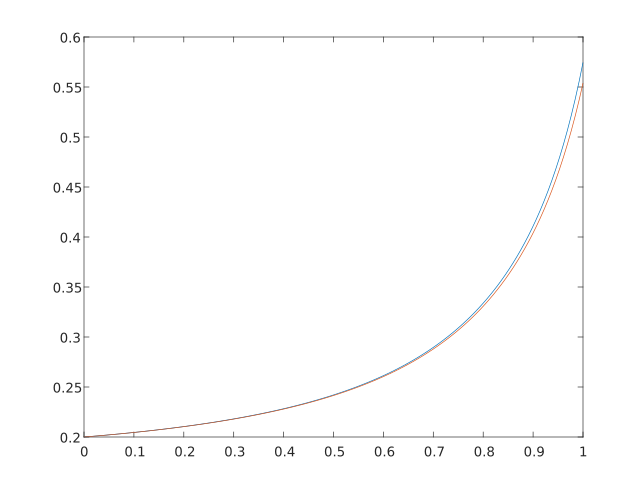
\includegraphics[width={\linewidth}]{plot_p9c.png}
				\caption{The solution of (\ref{eq:p9:c:ode}) (orange) and the numerical solution with $h=\frac{1}{128}$ (blue)}
				\label{fig:p9c}
			\end{figure}
			
			\questionpart We consider using the backward Euler method to solve
			\begin{equation}
				\label{eq:p9:d:ode}
				y' = e^{4t}y^2, \qquad y(0) = 0.1, \qquad 0\le t\le 1.
			\end{equation}
			Repeating the separation of variables in Problem 8 (c), we can find that
			\begin{equation}
				y(t) = \frac{4}{41 - e^{4t}}.
			\end{equation}
			Noting that $y(t) \to\infty$ as $t\to \frac{\log(41)}{4} \approx 0.9284 < 1$, we see that the solution $y$ of (\ref{eq:p9:d:ode}) actually only exists on an interval $\left[0, \frac{\log(41)}{4}\right)$, so when using the backward Euler method to solve on $[0,1]$, we expect something bad (or at least unpredictable) to happen near $t = 0.9284$.
			
			Indeed, running the numerical simulation, the numerical values start off approximating $y$ well, but then fail around $t = 0.9284$. Smaller values of $h$ allow the approximation to stay good for longer, but none of them make it past $t = 0.9284$. In Figure \ref{fig:p9d_h128} we can see the numerical solution with $h=\frac{1}{128}$ using Newton's method as the nonlinear solver. In Figure \ref{fig:p9d_h1000}, we can see that the numerical solution stays faithful a little longer when $h = \frac{1}{1000}$.
			
			\begin{figure}[H]
				\centering
				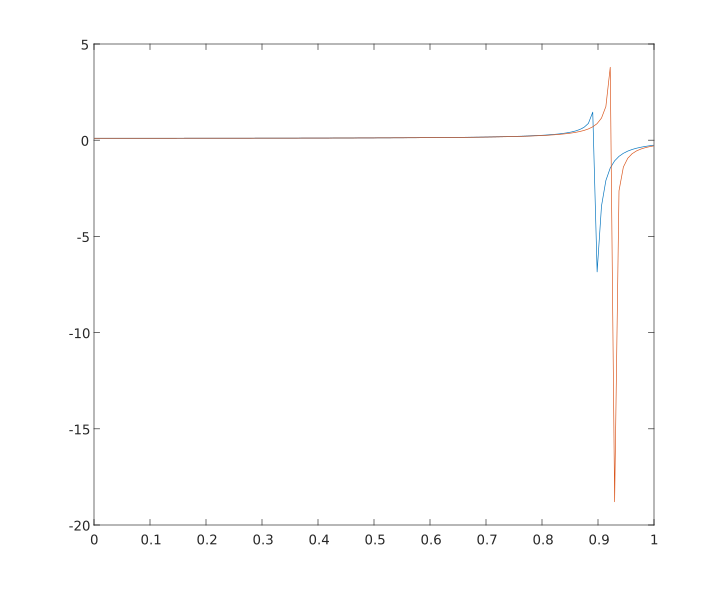
\includegraphics[width=\linewidth]{plot_p9d_h128.png}
				\caption{The solution of (\ref{eq:p9:d:ode}) (orange) and the numerical solution with $h=\frac{1}{128}$ (blue), using Newton's method as the nonlinear solver.}
				\label{fig:p9d_h128}
			\end{figure}
			
			\begin{figure}[H]
				\centering
				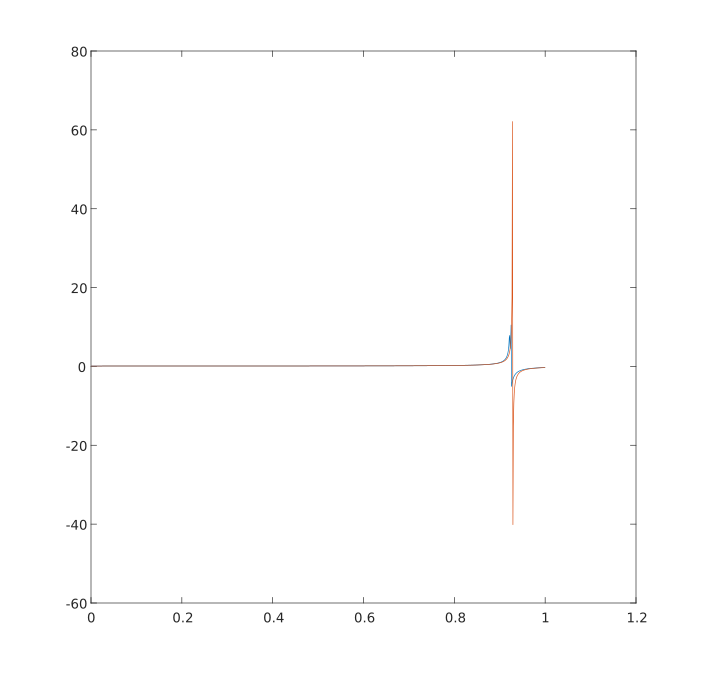
\includegraphics[width=\linewidth]{plot_p9d_h1000.png}
				\caption{The solution of (\ref{eq:p9:d:ode}) (orange) and the numerical solution with $h=\frac{1}{1000}$ (blue), using Newton's method as the nonlinear solver.}
				\label{fig:p9d_h1000}
			\end{figure}
			
			Using the fixed point method, the numerical solution blows up near the singularity (see Figure \ref{fig:p9d_fixed}). Interestingly, however, when using Newton's method and a sufficiently small step size $h$, the numerical solution doesn't blow up but jumps down near $t=0.9284$ and afterwards ``recovers'' and starts approximating a solution of the ODE again (albeit with a different initial condition). Newton's method fails to converge only on one step of the iteration when this happens. In the blow-up cases, the nonlinear solvers fail to converge on every step after $t=0.9284$ (see \verb*|p9_output.txt| for details).
			
			\begin{figure}[H]
				\centering
				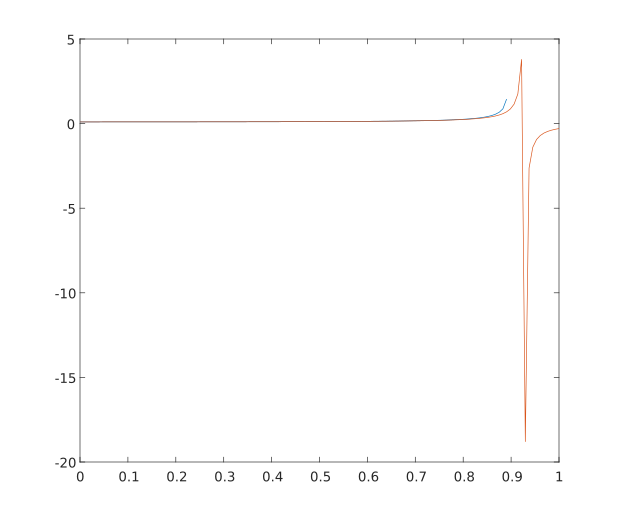
\includegraphics[width=\linewidth]{plot_p9d_fixed.png}
				\caption{The solution of (\ref{eq:p9:d:ode}) (orange) and the numerical solution with $h=\frac{1}{128}$ (blue), using the \textit{fixed point} method as the nonlinear solver. The numerical solution blows up to infinity near $t=0.9284$, so its graph is cut off on the step where it blew up.}
				\label{fig:p9d_fixed}
			\end{figure}
			
		\end{alphaparts}
\end{document}